\documentclass[12pt,a4paper,oneside]{article}
\usepackage[a4paper,left=3cm,right=2cm,top=2.5cm,bottom=2.5cm]{geometry}
\usepackage{graphicx}
\usepackage{lineno}
\usepackage{enumitem} 
\usepackage{lscape}
\usepackage{hyperref} 
\usepackage{apacite}
\usepackage{booktabs}
\usepackage{tikz}
\usepackage{bookmark}
\usepackage{multicol} 
\usetikzlibrary{shapes.geometric, arrows}

\tikzstyle{startstop} = [rectangle, rounded corners, minimum width=1.5cm, minimum height=1cm,text centered, draw=black, fill=red!30]
\tikzstyle{io} = [trapezium, trapezium left angle=70, trapezium right angle=110, minimum width=3cm, minimum height=1cm, text centered, draw=black, fill=blue!30]
\tikzstyle{process} = [rectangle, minimum width=3cm, minimum height=1cm, text centered, draw=black, fill=orange!30]
\tikzstyle{decision} = [diamond, minimum width=3cm, minimum height=1cm, text centered, draw=black, fill=green!30]
\tikzstyle{arrow} = [thick,->,>=stealth]



\begin{document}

\begin{sloppypar}

\begin{center}


\includegraphics[scale=0.30]{mmu.png}\\
\vspace{1cm}
\Large{\textbf{TDS 3301 \\Data Science Fundamentals}} \\
\vspace{2.5cm}
\Large{\textbf{PROJECT}} \\
\vspace{2.5cm}
 \Large{\textbf{Birds Classifier}} \\


\vspace{8.5cm}


\normalsize{Prepared by} \\
\vspace{2.5cm}
\large{\textbf{Mak Yen Wei, 1181203334, 018-9495849}} \\


\end{center}

\thispagestyle{empty}

\clearpage 

% ============================================
\section{Exploratory Data Analysis}

%=========================================
\subsection{Where to get the data?}
The datasets comes from a repository of birds images that's compiled on a kaggle repository. The kaggle dataset link an be found here: https://www.kaggle.com/datasets/gpiosenka/100-bird-species. The original datasets contains 450 species of birds, each containing around 150 images of the species, however running such big datasets might consume quite a plenty of computing resources, while we don't have that, so we decided to use a smaller dataset which contains only 20 species of birds, each containing around 100 images of the species. The slicing of the datasets is made possbile by a python script that we've customly made for this purpose. 

\subsection{What is the data all about?}
Our data set contains 20 bird species which included 3000 training images (150 images per species), 100 test images (5 images per species) and 100 validation images (5 images per species.) This is a very high quality dataset where there is only one bird in each image and the bird typically takes up at least 50\% of the pixels in the image. As a result even a moderatly complex model will attain training and testing accuracies in the mid 90% range.
All images are 224 X 224 X 3 color images in jpg format. Data set includes a train set, test set and validation set. The data structure is convenient if you use the Keras ImageDataGenerator.flowfromdirectory to create the train, test and valid data generators.
Images were gather from internet searches by species name. Once the image files for a species was downloaded they were checked for duplicate images using a python duplicate image detector program I developed. All duplicates detected were deleted in order to prevent their being images common between the training, test and validation sets.

After that the images were cropped so that the bird occupies at least 50\% of the pixel in the image. Then the images were resized to 224 X 224 X3 in jpg format. The cropping ensures that when processed by a CNN their is adequate information in the images to create a highly accurate classifier. Even a moderately robust model should achieve training, validation and test accuracies in the high 90\% range. Because of the large size of the dataset I recommend if you try to train a model use and image size of 150 X 150 X3 in order to reduce training time. 

All files were also numbered sequential starting from one for each species. So test images are named 1.jpg to 5.jpg. Similarly for validation images. Training images are also numbered sequentially with "zeros" padding. For example 001.jpg, 002.jpg ….010.jpg, 011.jpg …..099.jpg, 100jpg, 102.jpg etc. The zero's padding preserves the file order when used with python file functions and Keras flow from directory.

The 20 types of birds can be listed here:
American Redstart ,
Barred Puffbird,
Belted Kingfisher,
Cape May Warbler,
Cream Colored Woodpecker,
Crested Caracara,
Eastern Meadowlark,
Eastern Towee,
European Goldfinch,
Hoatzin,
Hoopoes,
Iberian Magpie,
Imperial Shaq,
Kookaburra,
Red Bellied Pitta,
Rufuos Motmot,
Taiwan Magpie,
Tree Swallow,
Violet Green Swallow,
White Tailed Tropic

%=========================================
\subsection{How to visualize the content?}

The visualtion of the data we've looked into is the number of images in each 20 classes. It is important to take note of the number of images in each column to be able to understand what sorts up datasets we're working with and how we should treat the dataset. For example, if the dataset is having a class imbalance problem, meaning number of images in all of the classes are not around the same, we should consider using some sort of data augmentation techniques to balance out the dataset. In our case, we can see that the distribution is quite balanced, but we figured having a perfectly balanced dataset is in fact a good idea. Therefore, in the next section, we'll be talking about how we've augmented the dataset to make it more balanced.

\begin{figure}[h]
\centering

\includegraphics[scale=0.10]{diagrams/data_description.png}
\caption{Bar Plot of images count for each class}
\end{figure}
The bar plot above shows the number of images in each class. As you can see, the distribution is quite balanced, but we figured having a perfectly balanced dataset is in fact a good idea. Therefore, in the next section, we'll be talking about how we've augmented the dataset to make it more balanced.

%=========================================
\subsection{What data transformation to the dataset?}
The only data transformation part of the project is shrinking the 450 species birds images into just 20 classes. The reason for this is because we don't have enough computing resources to run such a big dataset. The slicing of the datasets is made possbile by a python script that we've customly made for this purpose.

\subsection{What is the brightness distribution of the dataset?}
Investigating the brightness of the images in our dataset gives us a better understanding of the dataset. 

\begin{figure}[h]
\centering
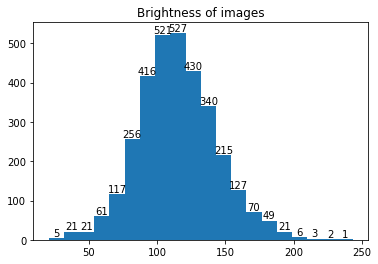
\includegraphics[scale=0.70]{color_distri.png}
\caption{Brightness Distribution}
\end{figure}

We can see that the brightness of the images are quite similar, which can be a good thing, and also a bad thing. The good thing is that we don't have to worry about the brightness of the images being too different from each other, The bad side of it is that the model will not be able to handle the brightness of the images that are too different from the training images. To counter this issue, there are several methods we can use, and in our finding, we used the ImageDataGenerator class from Keras to generate more images with different brightness, this is called data augmentation and will be explained in detailed in the later section 

\subsection{What is the color distribution of the dataset}
The color distribution of the dataset is also important to look into. The reason is because the color of the images can affect the model's performance. For example, if the model is trained on images with a lot of green, and then it is tested on images with a lot of red, the model will not be able to perform well. Another point of view is that if the color distribution between different classes are found to be unique and distinctive, that can help us to improve the model's performance by doing feature selection.

The following plot is to distinguish whether color is a telling factor in the classification of the birds. In the below exmaple we plotted 5 images of American redstart. 

\begin{figure}[h]
  \centering
  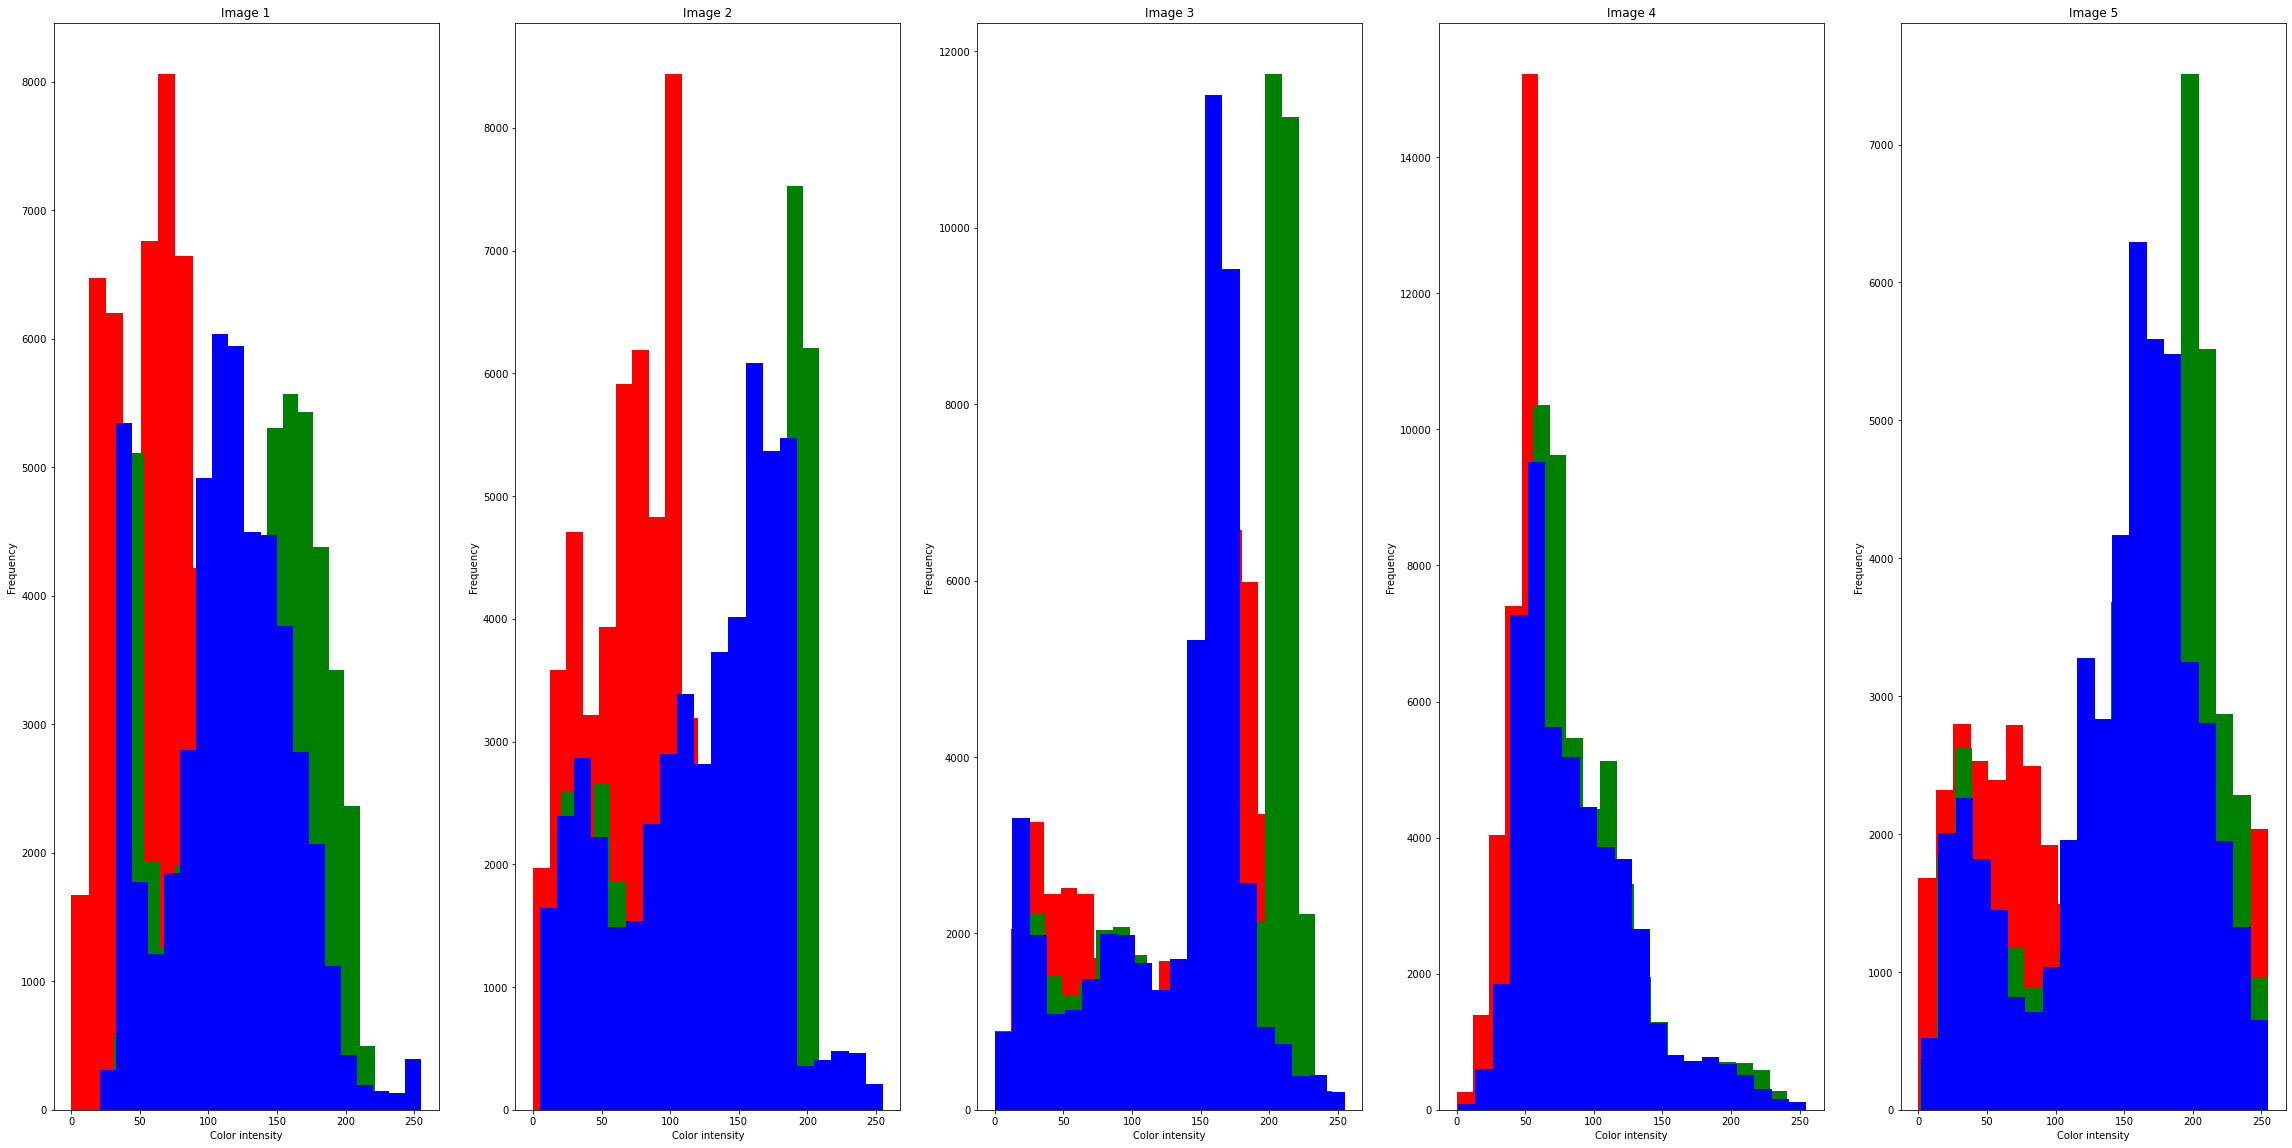
\includegraphics[scale=0.15]{brightness_distri.png}
  \caption{Color distribution }
  \end{figure}

In this case, we see that for american redstart, the blue channel tend to spike up, this might be a telling factor in the classification of the birds. Let's look at more plots to really solidifies our understanding of the color distribution of the dataset.

\begin{figure}[h]
\centering
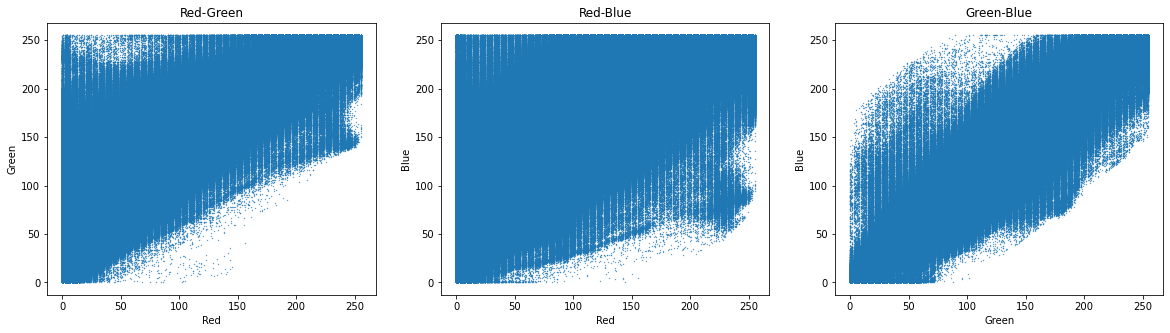
\includegraphics[scale=0.38]{cream-cloured-corr.png}
\caption{Cream Coloured WOODPECKER}
\end{figure}

\begin{figure}[h]
\centering
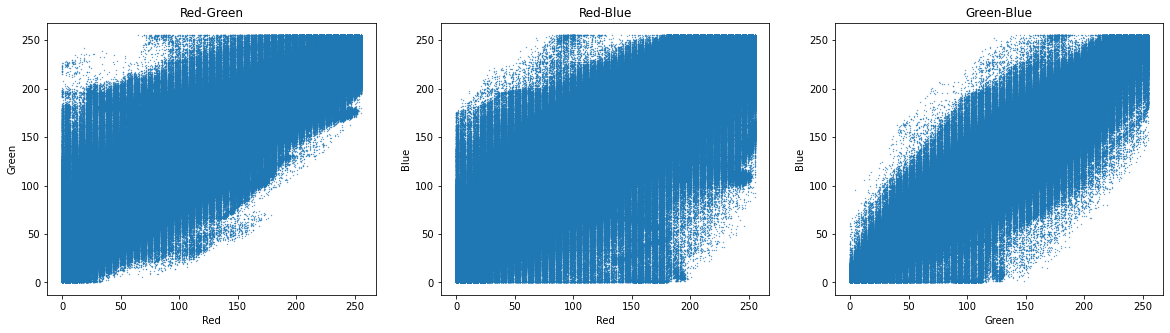
\includegraphics[scale=0.38]{kookaburra-corr.png}
\caption{KOOKABURRA}
\end{figure}

\begin{figure}[h]
\centering
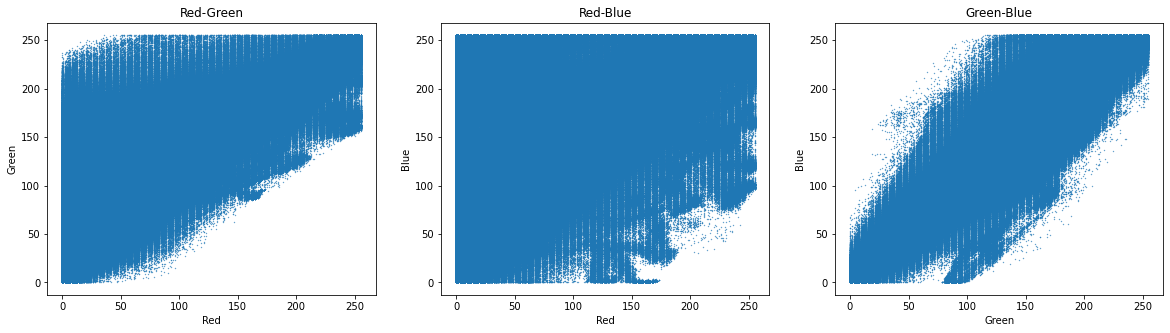
\includegraphics[scale=0.38]{campo-flicker-corr.png}
\caption{Campo Flicker}
\end{figure}

\begin{figure}[h]
\centering
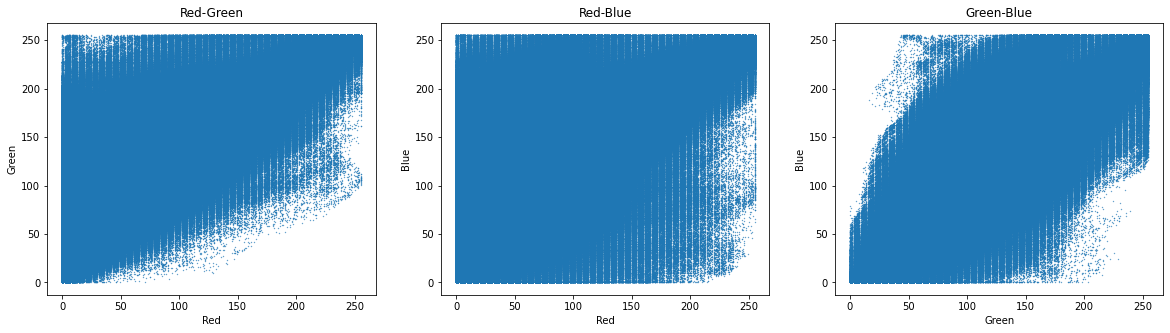
\includegraphics[scale=0.38]{rufuos-motmot-corr.png}
\caption{Rufous Motmot}
\end{figure}

\begin{figure}[h]
\centering
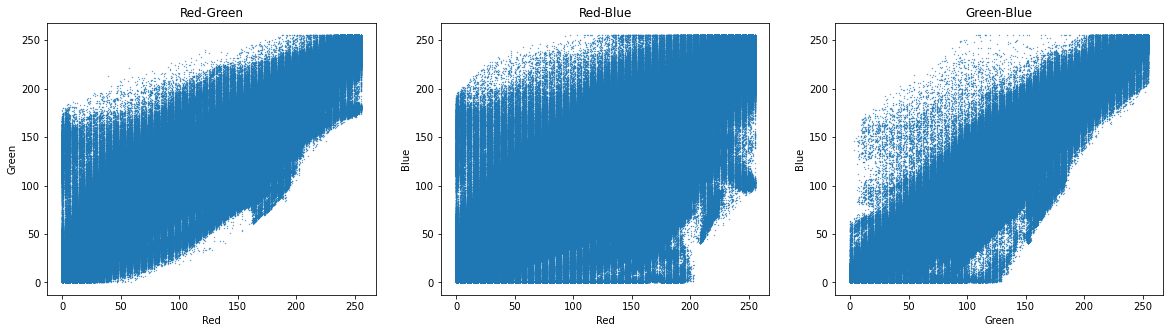
\includegraphics[scale=0.38]{white-tailed-tropic-corr.png}
\caption{White-tailed Tropicbird}
\end{figure}

As you might tell, the scatter plot of the color distribution of the images are quite similar to each other. This means that there are no distinctive color distribution between the classes which tells us that the color of the images are not a telling factor in the classification of the birds.

\pagebreak
\subsection{Size of the image?}
Next up, we look into the size of the images. Below we are plotting the size of one of the images in the dataset. The images are all in the same size, which is 224x224. This is because we are using the VGG16 model, which is a pre-trained model that is trained on images of size 224x224. However, if we are training it on the original size, you can see that the images are quite big, and it will take a lot of time to train the model. The bigger the image the larger the details, and the more time it takes to train the model. 

\begin{figure}[ht]
\centering
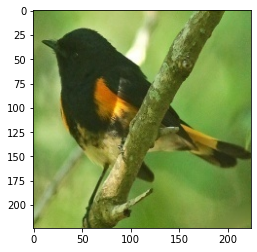
\includegraphics[scale=0.6]{size_demo.png}
\caption{Sizes of the images}
\end{figure}

In order to counter this issue, we attempt to use a gaussian blur filter to blur the images, and then resize it to 224x224. The reason for this is because we want to reduce the details of the images, and also reduce the size of the images.

\begin{figure}[h]
\centering
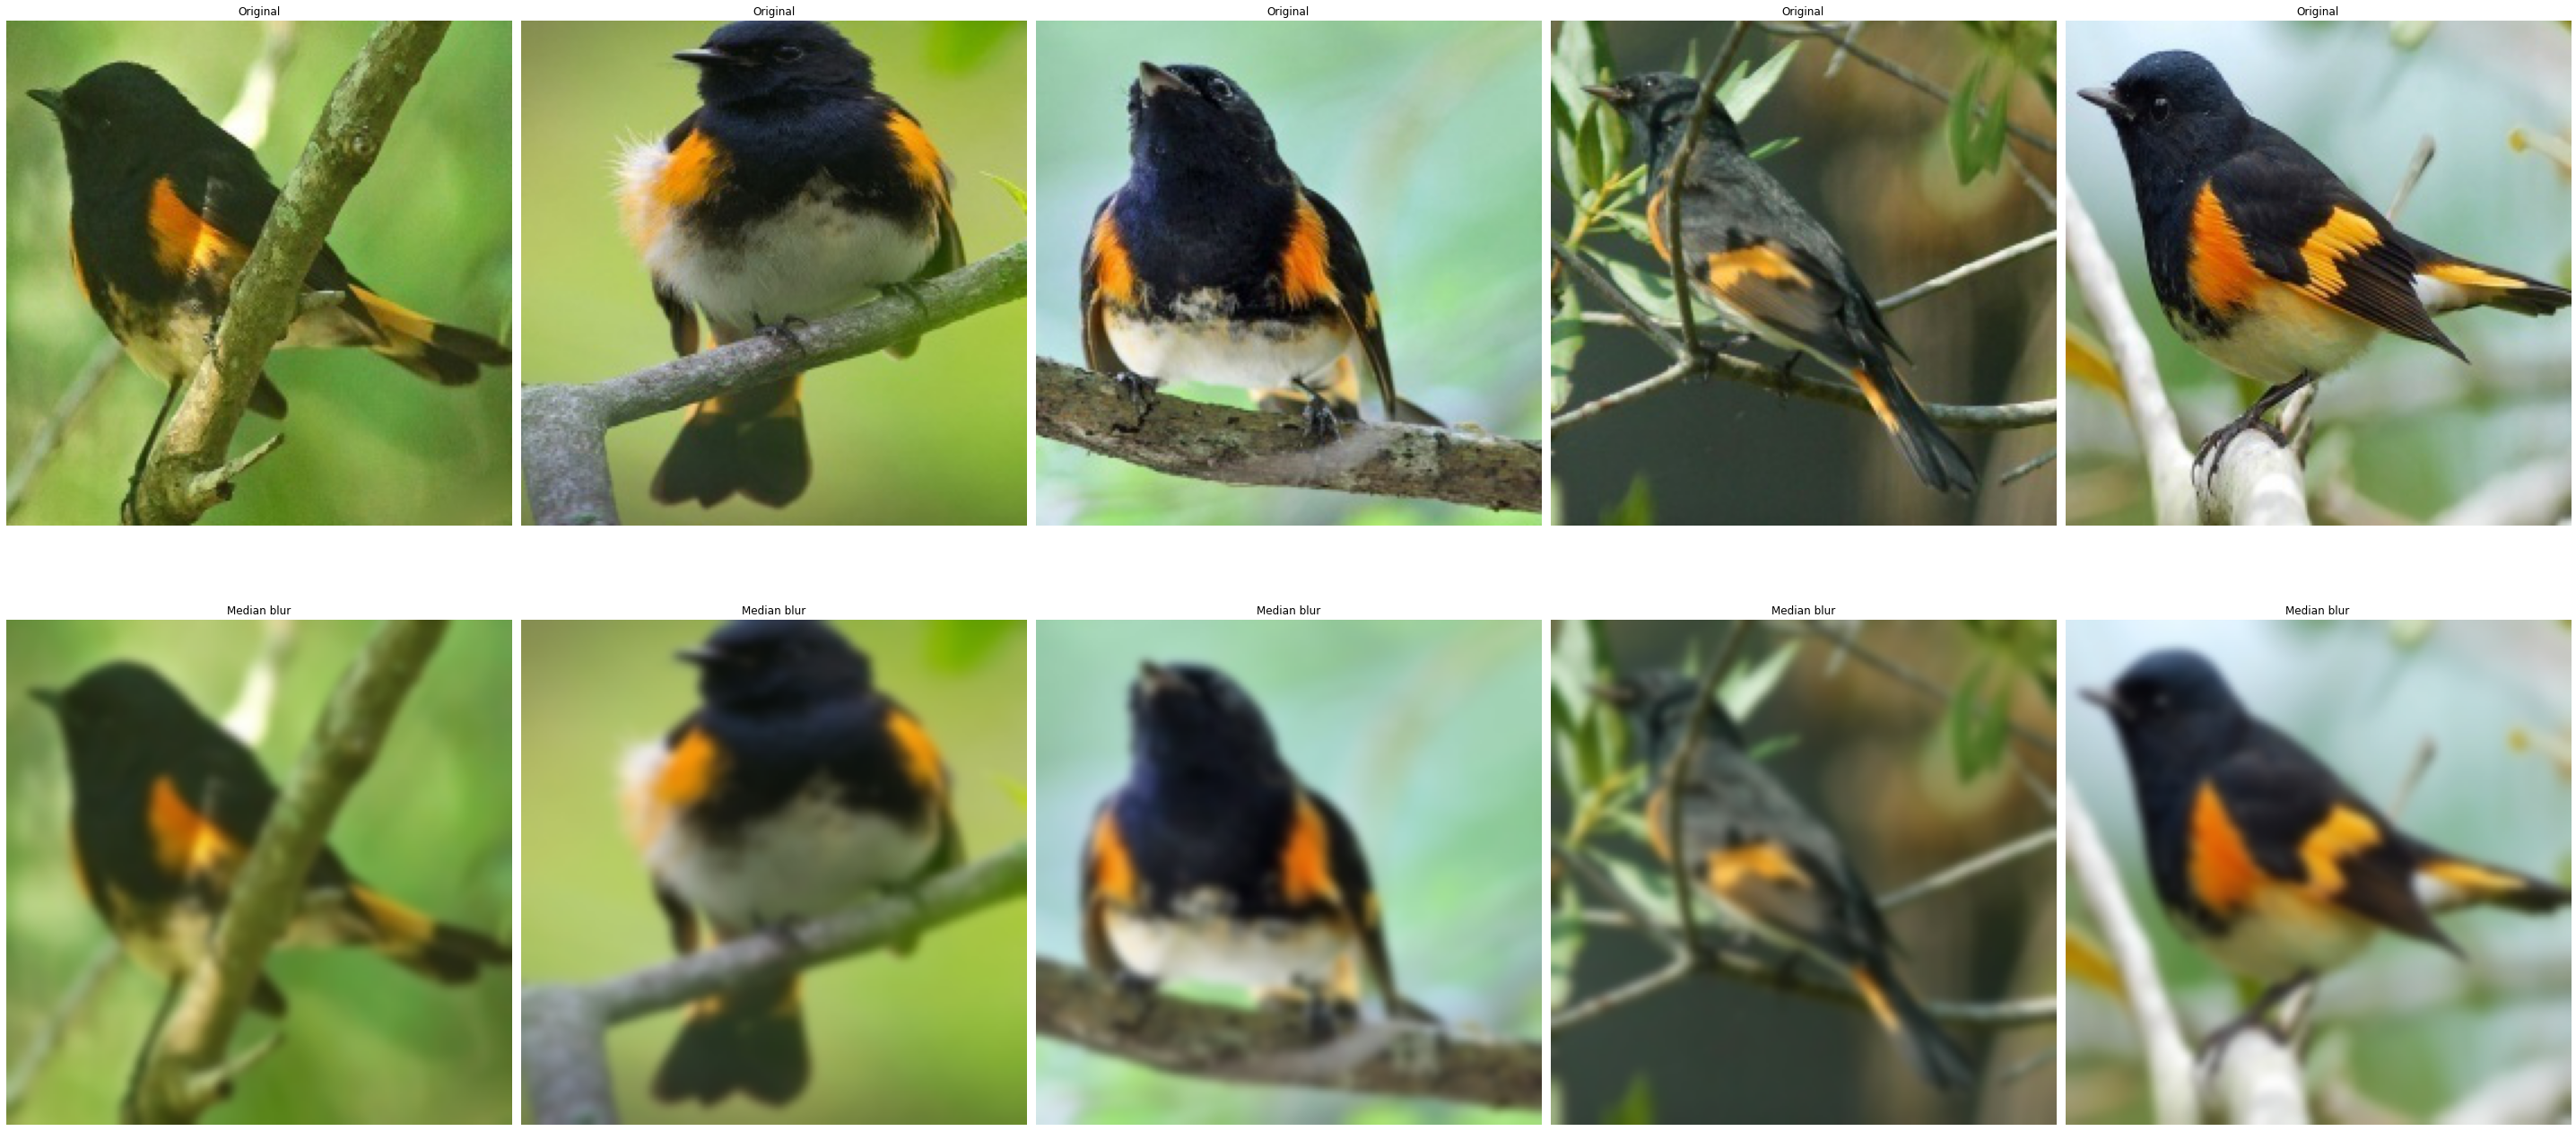
\includegraphics[scale=0.1]{gaussian_blur.png}
\caption{Gaussian blur comparison}
\end{figure}

The above figure shows a comparison between the original image and the blurred image. As you can tell, the details had been reduced by a lot. The gaussian distribution is a bell-shaped curve, and the center of the curve is the mean, and the width of the curve is the standard deviation. The standard deviation is the measure of how spread out the numbers are. The higher the standard deviation, the more spread out the numbers are. In this case, we are using a standard deviation of 5, which means that the numbers are quite spread out. 

\subsection{What can we predict, and how can we do that?}
The next step is to look into the dataset and see what we can predict. In this case, we are predicting the bird species, we'll be looking at 3 models which are VGG16, VIT and lastly MobileNet.

%=========================================
\pagebreak
\section{Pre-Processing Methods.}

\subsection{Rescale, Normalization}
Before we use the data for model training and inference, we can implement some pre-processing methods which are the steps taken to format the images. Firstly, for normalisation, we have to rescale the training data, validation data as well as test data.We rescale all of the data with the value 1/255. The reason is that our original images consist of RGB coefficients in the 0-255, but such values would be too high for our models to process (given a typical learning rate), so we target values between 0 and 1 instead by scaling with a 1/255 factor.

\subsection{Data Augmentation}
Data augmentation is a well-known technique to artificially create new training data from existing training data. It is useful to enhance performance and outcomes of a machine learning model by creating new and different training examples. For instance, image resizing, image rotation, image flipping and so on. Therefore, we are artificially expanding the available dataset for training the deep learning models which are all of the selected models. Additionally, we apply the technique only on training data not on validation data, nor on testing data. 

\subsection{Flipping, Rotation, Zooming, Brightness}
The data augmentation methods we are using is ImageDataGenerator in Keras. We have implemented a few augmentation techniques which are flipping, rotation and zooming. First of all, we set horizontal\_flip and vertical\_flip as true which let the image randomly flip half of the images horizontally and vertically. Secondly, image rotation allows the model to become invariant to the orientation of the object. In this case, we rotate the image by setting rotation\_range value between 0 to 180 degrees. Thirdly, the zoom augmentation either randomly zooms in on the image or zooms out of the image. For that, we set the zoom\_range with the value 0.1 to let it zoom inside the image. Lastly, we set brightness\_range for brightening or darken bird images. The value is set between 0.1 to 0.9.

The following is a plot of the augmented images. The original images are on the left and the augmented images are on the right. As you can see, the augmentation technique introduces skewness, rotation, brightness varities to the image. This will tremendously helps the model to learn the features of the images better and fit edge cases better.

\begin{figure}[h]
\centering
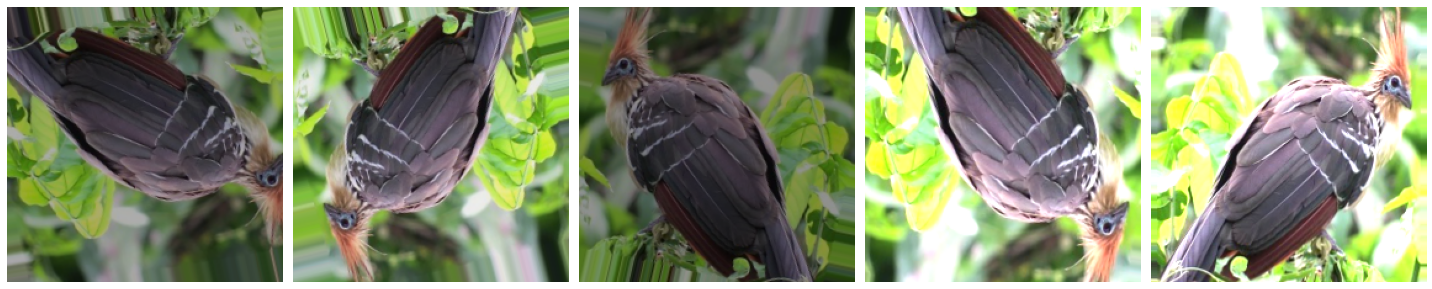
\includegraphics[scale=0.30]{brightness_enhancement.png}
\caption{Augmented Images}
\end{figure}

\pagebreak
\section{Model Construction and Comparison}
\subsection*{Models Used}
We have used 3 models which are VGG16, VIT and MobileNet. The reason for using these 3 models is because they are all pre trained models, and they are all state of the art models. The VGG16 model is a convolutional neural network that is trained on more than a million images from the ImageNet database. The VIT model is a vision transformer model that is trained on more than a million images from the ImageNet database. The MobileNet model is a convolutional neural network that is trained on more than a million images from the ImageNet database.

\subsection*{Model Training}
The model is primarily trained on 2 different metrics, Learning rate of 0.001 and 0.0001. All models are trained on epoch of 30 and the batch size of 32

\subsection*{Hyperparemeters Tuning} 
The hyperparameters that we are tuning are the learning rate, the optimizer, the activation function, the loss function and the metrics. The learning rate is the step size at each iteration while moving toward a minimum of a loss function. The optimizer is the algorithm used to update the weights of the neural network. The activation function is the function that is applied to the weighted sum of the inputs of a node. The loss function is the function that is used to evaluate a set of weights. The metrics is the function that is used to judge the performance of the model.


To ease our work, we came up with 2 functions, a function to tune the learning rate as the number of epoch passes, and a early stopping function. The learning rate function is used to reduce the learning rate as the number of epoch passes. The early stopping function is used to stop the training process when the validation loss is not decreasing anymore. To further understand the learning rate schedule, we first talk about the issue if you have a high learning rate, and a low learning rate. If you have a high learning rate, the model will converge faster, but it will not be able to find the global minimum. We can see that in the plot below

\begin{figure}[h]
\centering
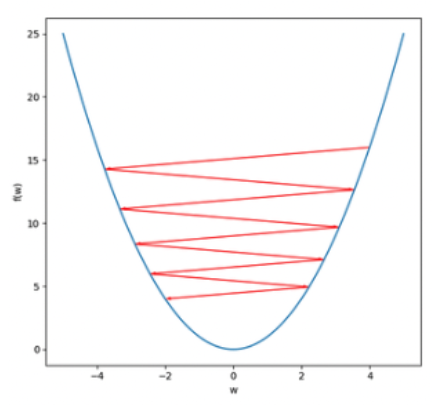
\includegraphics[scale=0.6]{lr-schedule-2.png}
\caption{Learning rate Plot}
\end{figure}

If you have a low learning rate, the model will converge slower, but it will be able to find the global minimum, which is a better way to train the model. We can see that in the plot below

\begin{figure}[h]
\centering
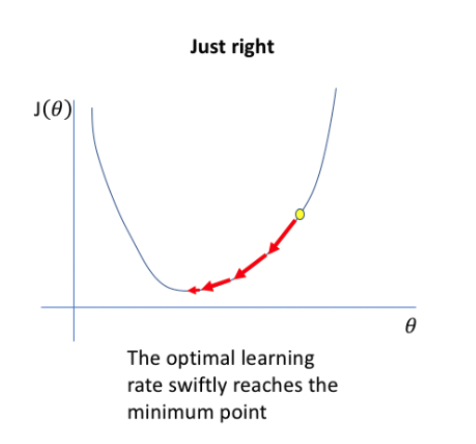
\includegraphics[scale=0.6]{lr-schedule.png}
\caption{Learning rate Plot}
\end{figure}

On the other hand, early stopping is a method that allows you to specify an arbitrary large number of training epochs and stop training once the model performance stops improving on a hold out validation dataset. The early stopping function is used to stop the training process when the validation loss is not decreasing anymore.

\subsection*{Model Evaluation}
\subsubsection*{VGG16}
VGG16 is a convolutional neural network that is 16 layers deep. The pretrained network can classify images into 1000 object categories, such as keyboard, mouse, pencil, and many animals. The network has an input image size of 224-by-224.

We can compare the model on different learning rates of 0.001 and 0.00001
\begin{figure}[h]
\centering
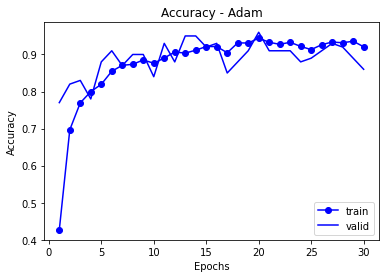
\includegraphics[scale=0.40]{diagrams/vgg16/0.001lr_graphs/Adam_acc.png}
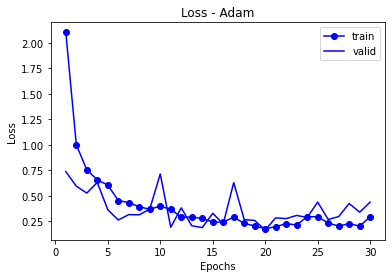
\includegraphics[scale=0.40]{diagrams/vgg16/0.001lr_graphs/Adam_loss.png}
\includegraphics[scale=0.40]{diagrams/vgg16/0.001lr_graphs/SGD_acc.png}
\includegraphics[scale=0.40]{diagrams/vgg16/0.001lr_graphs/SGD_loss.png}
\caption{Adam, SGD Acc,  Loss - Learning rate Comparison}
\end{figure}


The above plots are trained on the learning rate of 0.001

\pagebreak
\begin{figure}[h]
  \centering
  \includegraphics[scale=0.40]{diagrams/vgg16/0.0001lr_graphs/lr0.0001_Adam_acc.png}
  \includegraphics[scale=0.40]{diagrams/vgg16/0.0001lr_graphs/lr0.0001_Adam_loss.png}
  \includegraphics[scale=0.40]{diagrams/vgg16/0.0001lr_graphs/lr0.0001_SGD_acc.png}
  \includegraphics[scale=0.40]{diagrams/vgg16/0.0001lr_graphs/lr0.0001_SGD_loss.png}
  \caption{Adam, SGD Acc,  Loss - Learning Rate Comparison}
  \end{figure}

The above plots are trained on the learning rate of 0.0001.

As you can tell from the plot, the model with the learning rate of 0.001 is able to converge faster than the model with the learning rate of 0.0001. The model with the learning rate of 0.001 is able to achieve a higher accuracy than the model with the learning rate of 0.0001. The model with the learning rate of 0.001 is able to achieve a lower loss than the model with the learning rate of 0.0001. Also, the model using the Adam optimizer is able to achieve a higher accuracy than the model using the SGD optimizer.

\subsubsection{Model Performance Table | VGG16}
\begin{figure}[h]
  \centering
  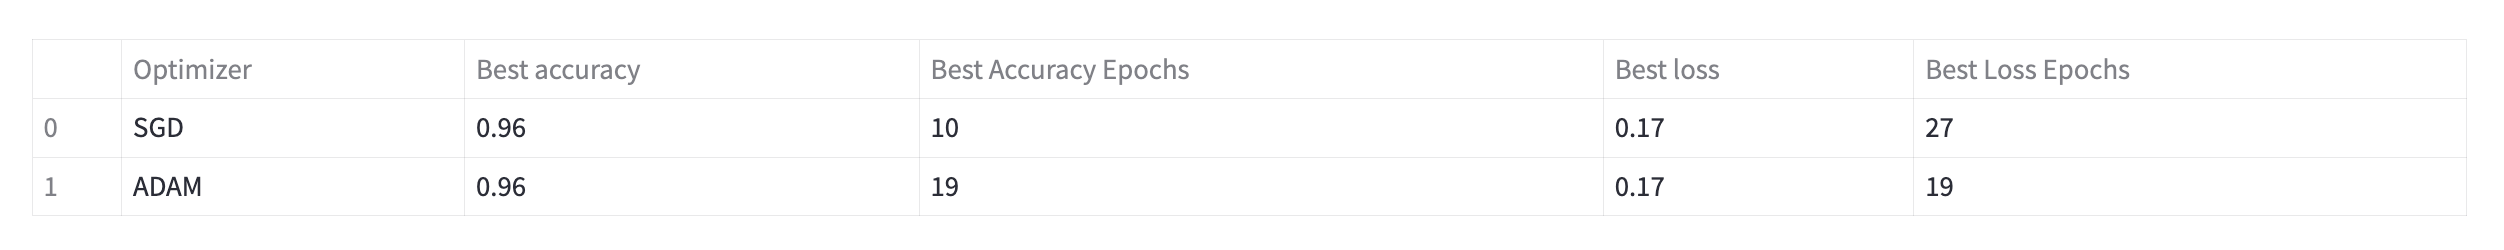
\includegraphics[scale=0.40]{vgg16-table.png}
  \caption{Model Performance Table Using VGG16}
  \end{figure}

\subsubsection*{Mobile Net}
Mobile Net is a convolutional neural network that is 16 layers deep. The pretrained network can classify images into 1000 object categories, such as keyboard, mouse, pencil, and many animals. The network has an input image size of 224-by-224.

We can compare the model on different learning rates of 0.001 and 0.00001
\begin{figure}[h]
\centering
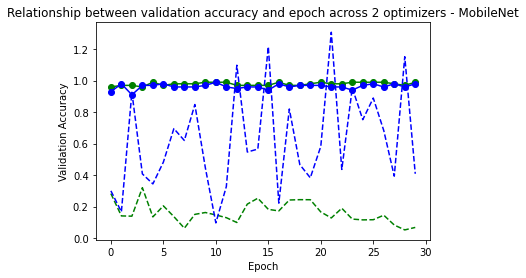
\includegraphics[scale=0.40]{diagrams/mobilenet/lr0.001_optimizer_compare.png}
\caption{Adam, SGD Acc,  Loss - Learning Rate Comparison}
\end{figure}


The above plots are trained on the learning rate of 0.001.

\pagebreak
\begin{figure}[h]
  \centering
  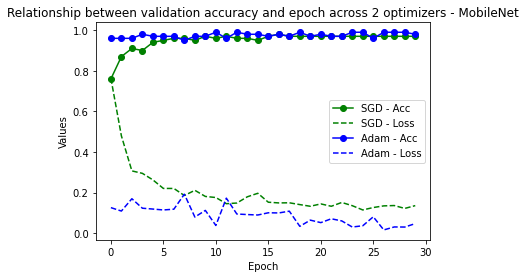
\includegraphics[scale=0.40]{diagrams/mobilenet/lr0.0001_optimizer_comparison.png}
  \caption{Optimizer Comparison using VGG16}
  \end{figure}

The above plots are trained on the learning rate of 0.0001,

The plots shows us that the learning rate of 0.0001 gives us a stable and smooth decent to the global minima, and both of the optimizers worked really well, achieveing a high accuracy and low loss.

\subsubsection{Model Performance Table | Mobile Net}
\begin{figure}[h]
\centering
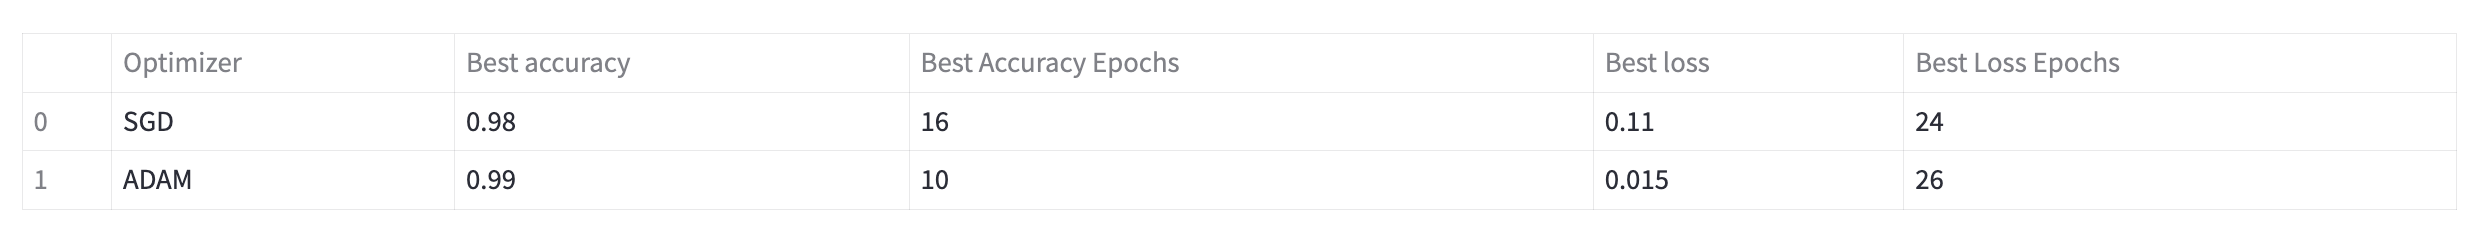
\includegraphics[scale=0.40]{mobile-net-table.png}
\caption{Model Performance Table Using Mobile Net}
\end{figure}


\subsubsection*{VIT}
The ViT is a visual model based on the architecture of a transformer originally designed for text-based tasks. The ViT model represents an input image as a series of image patches, like the series of word embeddings used when using transformers to text, and directly predicts class labels for the image.

\begin{figure}[h]
\centering
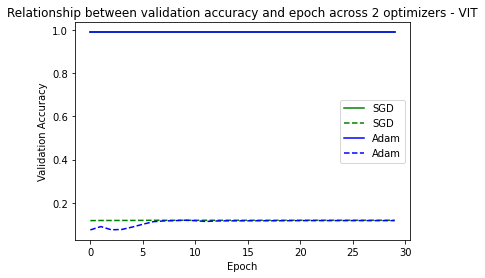
\includegraphics[scale=0.40]{diagrams/vit/optimizer_comparison.png}
\caption{Adam, SGD Acc,  Loss}
\end{figure}

With what we can understand from the above graphs, VIT is by far the best model we've tested, with a high accuracy and low loss, and both of the optimizers worked really well. 

\pagebreak
\subsubsection{Model Performance Table | VIT}
\begin{figure}[h]
  \centering
  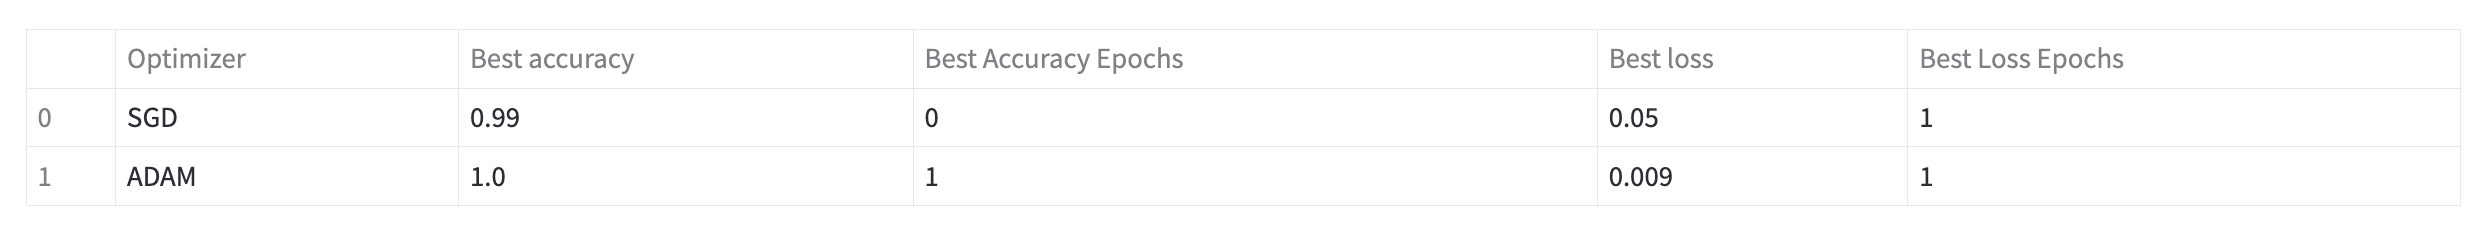
\includegraphics[scale=0.40]{vit-table.png}
  \caption{Model Performance Table Using VIT}
  \end{figure}

\subsection*{Conclusion}
After implementation of the model, we can evaluate it by comparing the resulting accuracy and loss. With computer resources as a concern in mind, in our opinion, we’ll look more towards the Best Validation accuracy and also the number epoch needed to achieve the results. With that being said, Vision Transformer (ViT) will be the best model for the image classification of bird species in this project. MobileNet will be ranked in second place which means it is better than VGG16 but worse than Vision Transformers (ViT). Lastly, VGG16 will be the last option which has the worst performance in this project.
\section{Deployment}

%=========================================
\subsection{How to connect to your web API?}
API is hosted here publicly: https://birds-classifier-api.herokuapp.com/

The API is hosted using a framework called FastAPI. We've extracted the best model --- VIT and saved it using joblib. The API is able to take in a image and return the prediction of the bird species.

However the api endpoint might not always be available to serve requests, if you are interested in using the API, this is due to the heroku is not a free product, and we are not able to keep it running 24/7. 

%=========================================
\subsection{Hosted streamlit?}
Streamlit is hosted here publicly: https://shaunmak-birds-classifier.streamlit.app/

The streamlit application contains all of our findings in a more detailed format, feel free to look it through.

%=========================================
\subsection{Do I have real-time prediction and visualization?}
Yes both API and Streamlit provides real time prediction but only streamlit application provides visualization

%=========================================
\subsection{How should I improve the performance? What strategy?}
There are primarily three things we hope to improve in the future.

As we know, one of the strengths of Transformer models is their flexibility to scale to high parametric complexity. Scaling up on compute, model and size of training samples improves performance only large models can benefit from more training data, and the performance of smaller models plateaus quickly and cannot leverage from additional data. This indicates that large scale models have the capacity to further enhance their representation learning capabilities. However, with the current designs, scaling upon Transformer models is expensive and compute prohibitive, thus an efficient design is required.

We would like to suggest that it reduces the high complexity of Transformer models. For example, explore selective or sparse attention to previous layer tokens while updating each next layer token. The Reformer model employed locally-sensitive hashing (LSH) to minimise the complexity of self-attention from O(n2) to O(nlog(n)). In similar pursuit, the recent Lambda Networks propose to model local context as a linear function which helps reduce complexity of self-attention.

Thirdly, we might face the problem of the object not always being in the center of the image, hence we can shift the pixels of the image either horizontally or vertically to overcome it. This can be done easily with the API which keras provides, namely “ImageDataGenerator”, by adding a parameter called “shift”. 
  

%=========================================

% Provide a detailed discussion about the process flow in EDA. Use a diagram to help in explanation. In this section you need to perform thorough analysis into the data such as missing value checking, imbalance data check, correlation analysis using various types of chart, data encoding methods and many more... 

% \begin{tikzpicture}[node distance=2cm]
% \node (start) [startstop] {Start};
% \node (in1) [io, right of=start, xshift=0.5cm] {Input};
% \node (pro1) [process, right of=in1, xshift=1.5cm] {Process 1}; 
% \node (dec1) [decision, right of=pro1, xshift=1.5cm] {Decision 1};
% \node (pro2a) [process, right of=dec1, xshift=1.7cm] {Process 2a};
% \node (pro2b) [process, above of=dec1, yshift=1cm] {Process 2b};
% \node (out1) [io, below of=pro2a] {Output};
% \node (stop) [startstop, below of=out1] {Stop};

% \draw [arrow] (start) -- (in1);
% \draw [arrow] (in1) -- (pro1);
% \draw [arrow] (pro1) -- (dec1); 
% \draw [arrow] (dec1) -- node[anchor=north] {yes} (pro2a);
% \draw [arrow] (dec1) -- node[anchor=east] {no} (pro2b);
% \draw [arrow] (pro2b) -- (pro1);
% \draw [arrow] (pro2a) -- (out1);
% \draw [arrow] (out1) -- (stop);


% \end{tikzpicture}

% \section{Feature Selection}

% In this section, you must discuss what are the 2 types of feature selection techniques used. How you actually combine them? How you look for the optimal features? Discuss why a certain set of features outperformed others? What is your recommendation/conclusion? ...etc

% \section{Model Construction \& Comparison}

% In this section, you firstly should discuss why you select a particular model. Why? Answer this first. Then, discuss the performances of models under different settings. You must provide a table for different settings, such as:

% \begin{table}[h]
% \begin{tabular}{|l|l|}
% \hline
% Experiment & Parameter Setting          \\ \hline
% $\xi1$         & depth = 3, leaf nodes = 10 \\ \hline
% $\xi2$          & ...etc                     \\ \hline
% $\xi3$         & ...etc                     \\ \hline
% \end{tabular}
% \end{table}

% Provide also a ROC for comparison.
% You should add more. Above is just some ideas for your to get things started!

% \section{Model Deployment}

% The models developed has been deployed at http://????
% The sample screenshots are given below:

% \begin{figure*}[h]
% \begin{multicols}{2}
%     
\includegraphics[width=\linewidth]{mmu.png}\par 
%     
\includegraphics[width=\linewidth]{mmu.png}\par 
%     \end{multicols}
% \begin{multicols}{2}
%     
\includegraphics[width=\linewidth]{mmu.png}\par
%     
\includegraphics[width=\linewidth]{mmu.png}\par
% \end{multicols}
% \caption{Screenshot of Streamlit}
% \end{figure*}

\end{sloppypar}
\end{document}